\chapter{Classifier Models}
\label{ch:chapter04}
 
%
% Section: 5 - Intro
%

Extraction of information about a software can be done following various approaches. In the past, rudimentary approaches such as searching for a term in paper, manual content analysis using human readers as well as rule based approaches have been employed \citep{kruger2019literature}. Recently, a deep learning model have also been employed for automatic extraction of  information about software such as mention types, software type, etc. \citep{schindler2022role}.  \\

Software is a real world entity and extraction of information about software can be approached as a named entity recognition problem. \ac{NER} tasks are one of classical sequence labeling tasks of NLP among others such as \ac{POS} tagging and text chunking \citep{akhundov2018sequence, he2020survey}. Therefore, automatic classification of software usage purpose can be approached as a sequence labeling task in which a class label, from a fixed list of class labels, is assigned to each token in a sequence. \\

Various types of sequence labeling models can be broadly categorized as statistical machine learning based or neural network based models \citep{he2020survey}. Classical machine learning based models for sequence labeling are \ac{HMM} \citep{kupiec1992robust}, \ac{MEMM} \citep{mccallum2000maximum}, and \ac{CRF} \citep{lafferty2001conditional}. These models are statistical and fundamentally depend on manually crafted features, external resources such as gazetteers and fail to adapt to new domains \citep{ma2016end}.   \\

In contrast, there are various neural network architectures and models that suit sequence labeling. \ac{RNN}, based on \ac{LSTM}, had been well established models for sequence labeling. Recently, transformer based neural network architectures, such as  \ac{BERT}, have pushed state-of-the-art performance further not only in sequence labeling tasks but for most \ac{NLP} tasks \citep{vaswani2017attention}. \\

This section presents and compares various types of sequence labeling models suitable for sequence labeling task of automatic classification of software usage purposes. 

\section{Machine learning Models}
\label{sec:chapter05:MLModels}

\subsection{Hidden Markov models (\ac{HMM}s)}
\label{sec:chapter05:MLModels:HMMS}

One of basic machine learning models that are used for sequence labeling are Hidden Markov Models. HMMs are based on Markov processes which describes a sequence of hidden finite states (Yi) in which a given state in a sequence depends only on the state prior to it \citep{aggarwal2018machine, gagniuc2017markov}. \\

The Markov chain of hidden states Yi generate observations Xi based on its current state using a joint probability distribution P(Y, X). The joint probability P(Y, X) is a product of conditional probability  P(X|Y) and a prior probability P(Y).  \\

\begin{figure}[htbp]
	\centering
	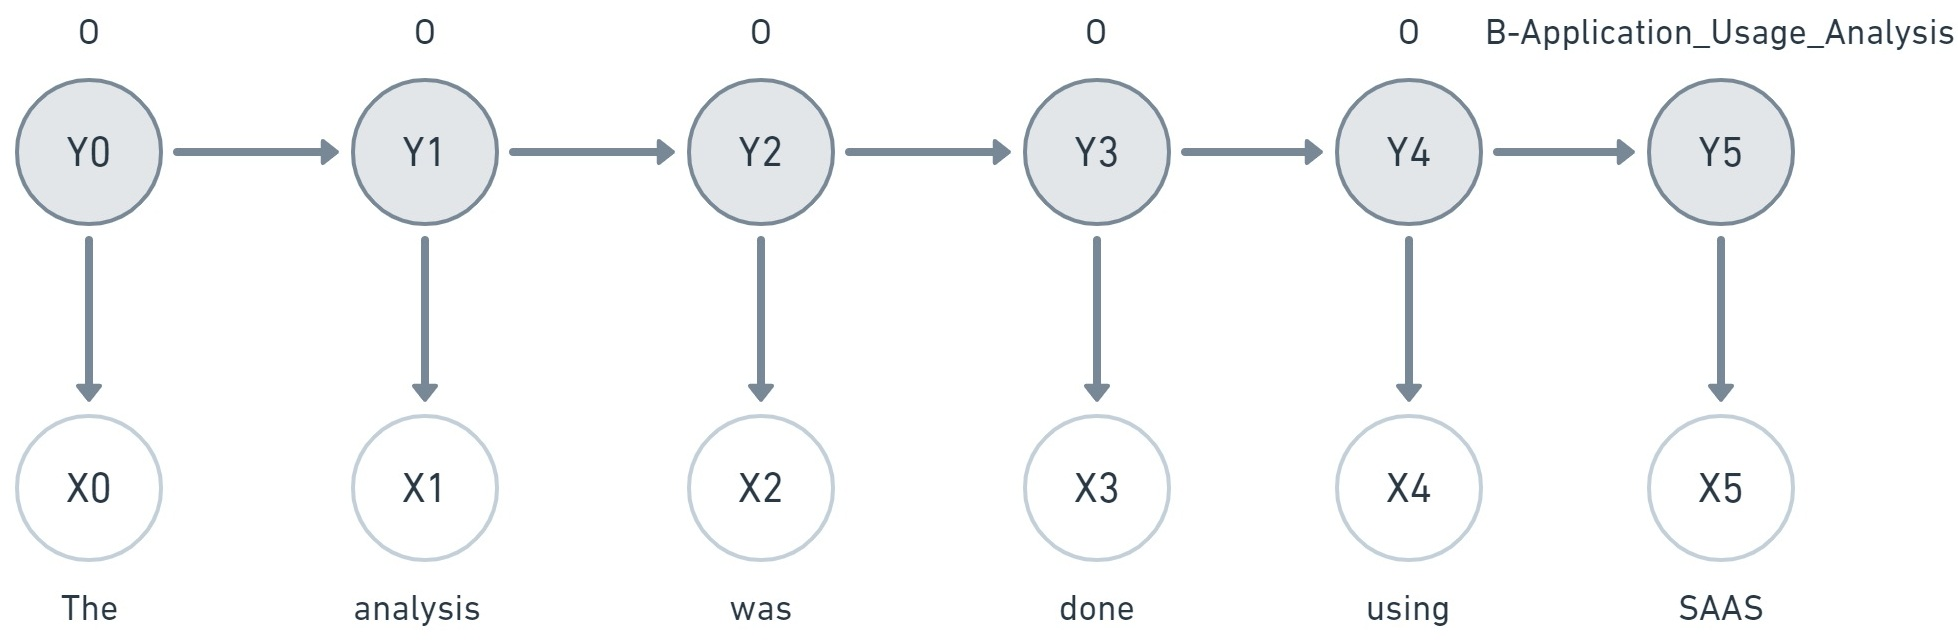
\includegraphics[width=.75\textwidth]{4.graphics/figures/ch_5/HMM}
	\caption{\ac{HMM} Model: a directed graph indicates generation of tokens depends on exactly the state before.}
	\label{fig:chapter03:setup}
\end{figure}

As the model transitions through hidden states of Yi, it generates an observation Xi which corresponds to a token in a sentence, hence HMMs are also referred to as generative models \citep{aggarwal2018machine}. \\

The challenge with Hidden Markov Models is that, it could be difficult to define the joint probability for some real world applications where the number of hidden states is infinite. In addition, Hidden Markov Models fail to capture long range dependencies because of their Markov assumption which considers only prior states \citep{bulla2006application, wallach2004conditional}.
 
\subsection{Maximum Entropy Markov Models (\ac{MEMM}s)}
\label{sec:chapter05:MLModels:MEMMs}

Unlike hidden Markov models which generate sequences of tokens based on hidden states, maximum entropy models are discriminative models i.e., they directly model the probability of each label Yi based on the current observation Xi and the prior hidden state Yi-1 \citep{mccallum2000maximum}. 

\begin{figure}[htbp]
	\centering
	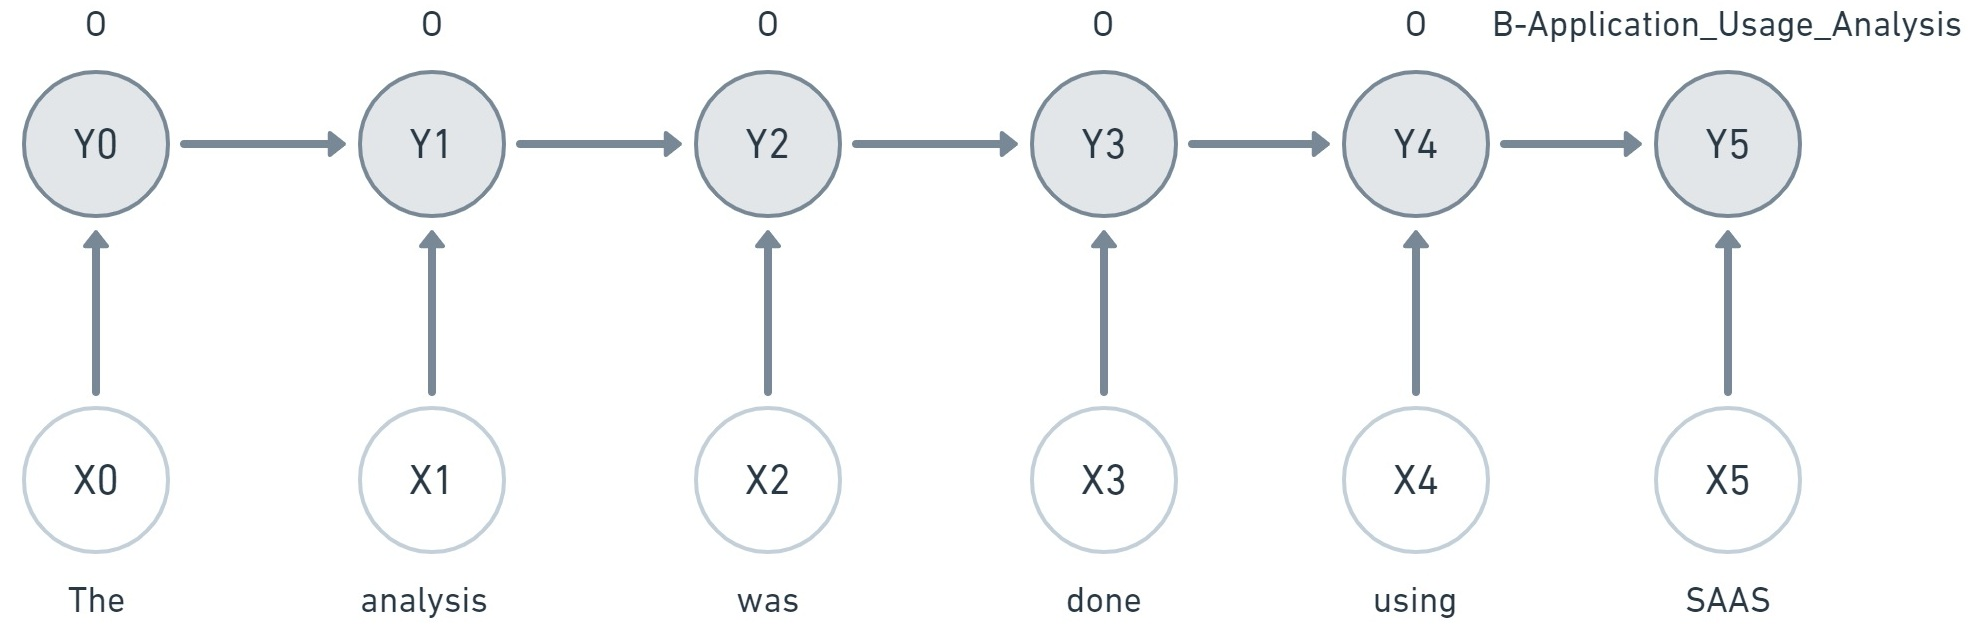
\includegraphics[width=.75\textwidth]{4.graphics/figures/ch_5/MEMM}
	\caption{MEMMs classify each token based on current observation and previous label}
	\label{fig:chapter03:setup}
\end{figure}

The biggest drawback with MEMMs and other discriminative directed graphical models based on Markov, tend to be biased in favor of states with fewer successor states i.e. \citep{lafferty2001conditional}. 

\subsection{(Linear) Conditional Random Fields (\ac{CRF}s)}
\label{sec:chapter05:MLModels:CRFs}

Conditional Random Fields are similar with \ac{MEMM}s in that both are probabilistic and discriminative models that can perform sequence labeling based on conditional probability P(Y|X) unlike joint probability of \ac{HMM}s \citep{wallach2004conditional}. A sequence of tokens in a sentence corresponds to X and Y refers to a sequence of class labels \citep{lafferty2001conditional}. 

\begin{figure}[htbp]
	\centering
	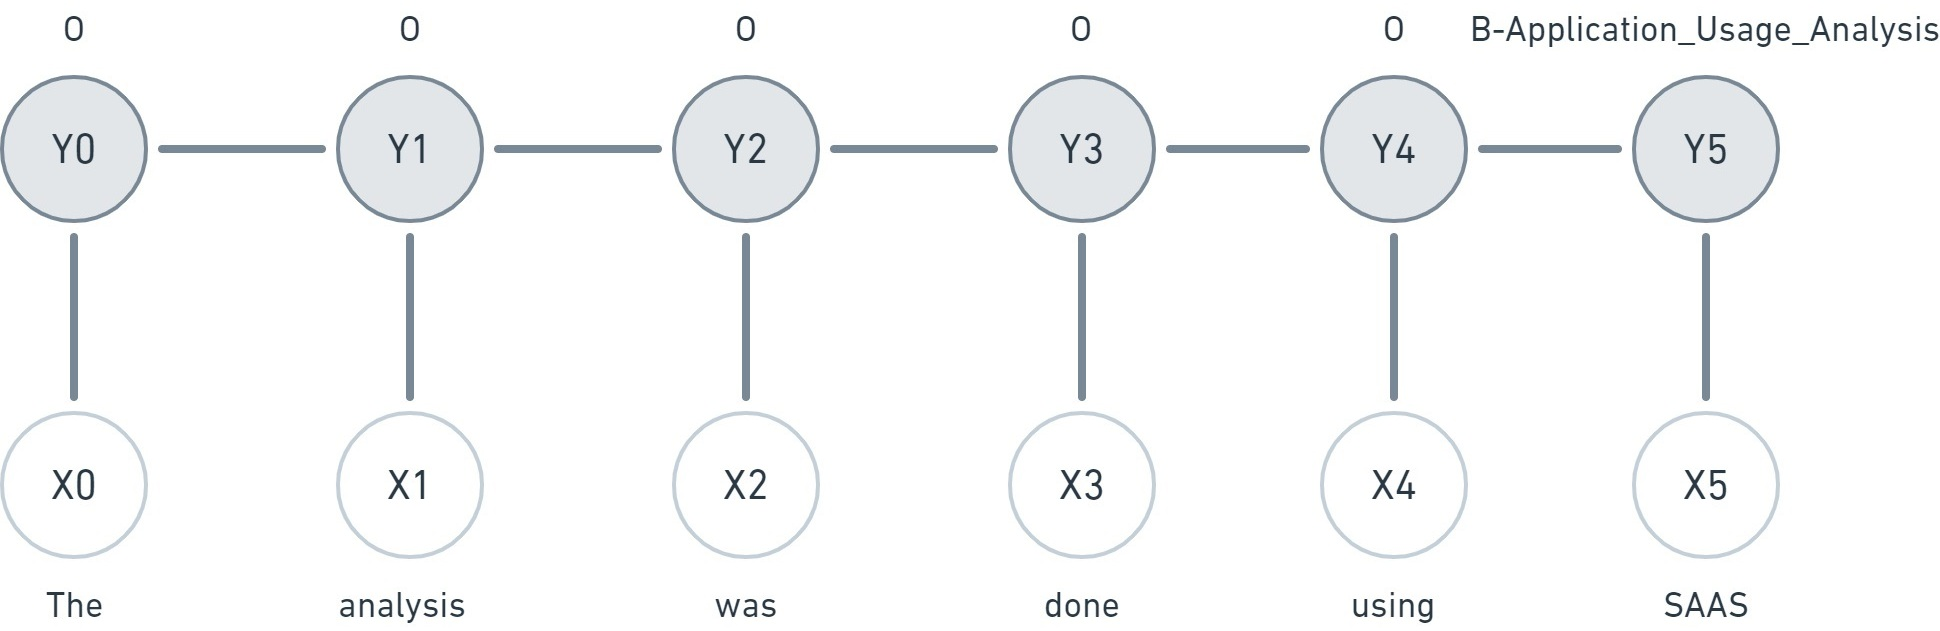
\includegraphics[width=.75\textwidth]{4.graphics/figures/ch_5/CRF}
	\caption{\ac{CRF} Model: un-directed graph indicates that classification at a given instance depends on labels occurring before and after.}
	\label{fig:chapter03:setup}
\end{figure}

\ac{CRF}s differ from \ac{MEMM}s in that they are undirected graphs, i.e., the inference of Yi depends on all the labels occurring before it as well as after it. This makes training of CRFs computationally expensive especially when a wider window of tokens is chosen to handle long range dependencies \citep{aggarwal2018machine}. 

\section{Deep Learning Models }
\label{sec:chapter05:MLModels:DLMs}

Deep learning based models are state-of-the-art for many machine learning and \ac{NLP} tasks, including sequence labeling. There are various types of deep learning architectures that suit for sequence labeling. Popular neural network architectures for sequence labeling tasks are recurrent neural networks and  transformer networks. \\

 
Recurrent neural network based models such as \ac{LSTM}, \ac{Bi-LSTM}, \ac{Bi-LSTM-CRF} had been state-of-the-art sequence labeling models, before the inception of transformer-encoder based models like BERT which produced a new state-of-the-art performance for many \ac{NLP} tasks including sequence labeling. 


\subsection{Long Short-Term Memory (\ac{LSTM})}
\label{sec:chapter05:DLModels:LSTM}


\ac{RNN}s are specific type of neural network architectures that take a sequence of inputs features to  yield a sequence of labels. However, plain RNNs fail to capture long-range dependencies because of vanishing and exploding gradient problems \citep{pascanu2013difficulty, fischer2018deep}. \\

Fortunately, other variants of RNNs such as LSTM networks are capable overcoming unstable gradient problems \citep{akhundov2018sequence, lample2016neural, ma2016end}. This is because, unlike RNNs, LSTM networks have memory cells that are composed of three gateways which determine what amount of information to forget at a given instant of time \citep{ma2016end}. \\

LSTM networks are typically composed of input layer, hidden layer(s), and output layer. Number of inputs to the input layer corresponds to input features and the number of outputs on the output layer corresponds to number of classes of the classification task. The memory cells of LSTM are found in the hidden layers of the network \citep{fischer2018deep}. A memory cell structure is depicted on the figure 5.4 below. 

\begin{figure}[htbp]
	\centering
	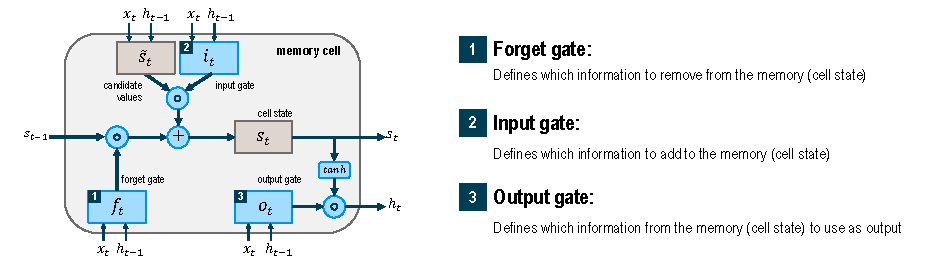
\includegraphics[width=1\textwidth]{4.graphics/figures/ch_5/pdf/LSTM_cell2}
	\caption{\ac{LSTM} Cell \citep{fischer2018deep}}
	\label{fig:chapter03:setup}
\end{figure}


\subsection{Bi-Long Short-Term Memory (\ac{Bi-LSTM})}
\label{sec:chapter05:DLModels:BiLSTM}

For sequence labeling tasks, it is desirable to access left as well as right input features to capture context information. However, LSTM models are capable of remembering only past (left) sequence of features.  \\

To solve this problem, Bi-LSTM combines two LSTM networks where the first LSTM unit captures  input features in a forward direction while the other captures the information in the reverse direction. Finally the two input features get concatenated to create a feature representation that encapsulates context information in both directions \citep{ma2016end}. 


\subsection{\ac{Bi-LSTM-CRF}}
\label{sec:chapter05:DLModels:BiLSTMCRF}

In sequence labeling, it is also important to capture correlations among adjacent input features at a sentence level. Since CRFs are capable of incorporating correlations among neighboring input features in a seqence, outputs of Bi-LSTM can be fed into CRF to create Bi-LSTM-CRF model which is aware of correlation between neighboring features in addition to context in both directions \citep{ma2016end}. \\

The use of past and future inputs using Bi-LSTM combined with CRF to capture correlations among features at a sentence level boosts sequence labeling accuracy. Because of this the Bi-LSTM-CRF model produce state-of-the-art results among LSTM based models. For example, an F1 score of 97.55\%, 94.46\% and 88.83\% is achieved on classical sequence labeling tasks of POS, chunking (CoNLL 2000) and NER (CoNLL-2003) respectively \citep{huang2015bidirectional}. 
 

\begin{figure}[htbp]
	\centering
	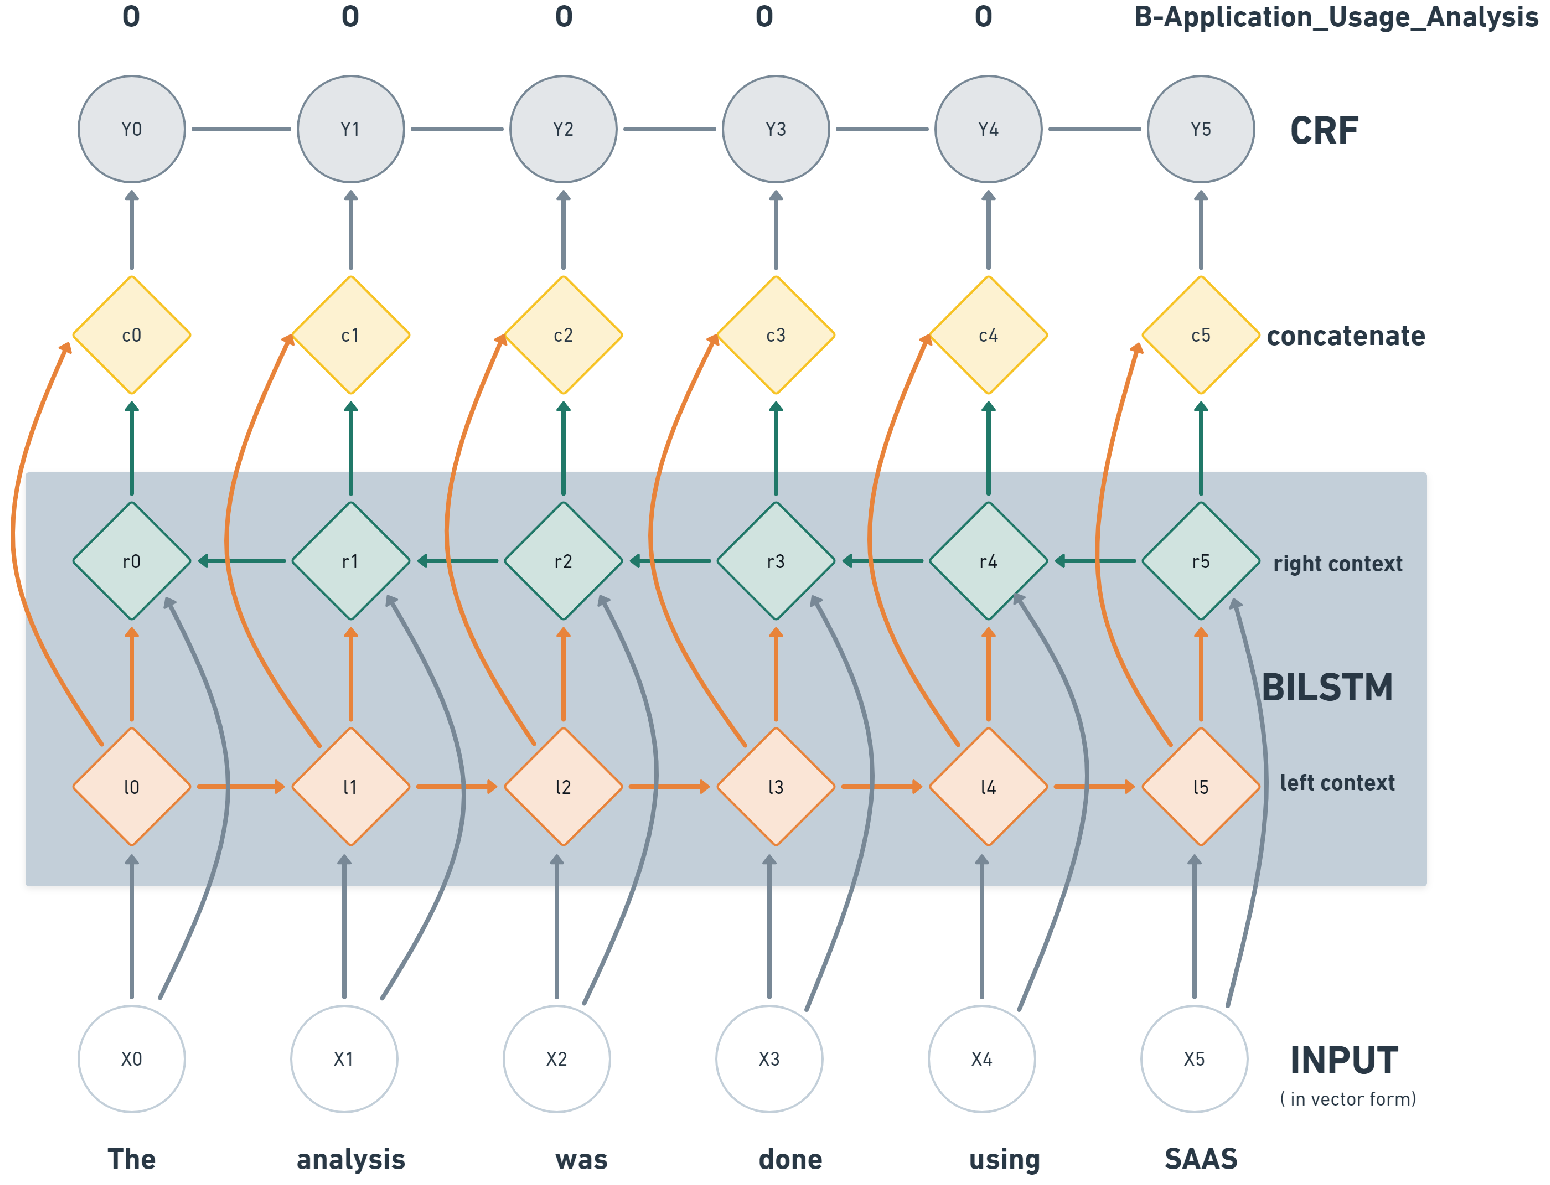
\includegraphics[width=.85\textwidth]{4.graphics/figures/ch_5/Bi-LSTM-CRF}
	\caption{A \ac{Bi-LSTM-CRF} model: the \ac{Bi-LSTM} layer captures context information in two directions from left to right and vice versa. }
	\label{fig:chapter03:setup}
\end{figure}

\section{Transformer based models}
\label{sec:chapter05:DLModels:Transformer}

Although Bi-LSTM-CRF models have superior performance for sequence labeling, over other LSTM based models, they have inherent weaknesses. Firstly, Bi-LSTM-CRFs are not truly bi-directional context readers, rather  pseudo-directionality is achieved learning right and left contexts separately and concatenating them. Because of this the true context of words could be lost slightly. \\

Secondly, Bi-LSTM-CRFs are very slow to train because of their sequential nature which does not allow to take  advantage of parallelization using \ac{GPU}s.  Third, training of Bi-LSTM-CRFs, like any other deep learning models, requires a lot of data and training models from scratch is computationally expensive. \\


The latest deep learning models based on transformer architectures are capable of overcoming shortcomings of Bi-LSTM-CRFs. First, transformer based models employ transfer learning where knowledge gained from pre-training can be re-used and fine tuned to solve specific problems \citep{ezen2020comparison}. In addition, transformer architectures have the ability to read past and future context simultaneously unlike Bi-LSTM-CRFs \citep{devlin2018bert}. Moreover, unlike LSTM networks, transformer models can handle sequential data simultaneously which gives the opportunity to expediate model training by parallelizing with the help of modern \ac{GPU}s \citep{ezen2020comparison}. 

\subsection{Bidirectional Encoder Representations from Transformers (\ac{BERT})}
\label{sec:chapter05:DLModels:Transformer:BERT}

BERT is state-of-the-art transformer based model with transfer-learning capability i.e. it can be pre-trained with unlabeled data and fine-tuned further for downstream applications just by adding one output layer \citep{devlin2018bert, ezen2020comparison}. \\

BERT is also referred to as \ac{MLM} because, the model arbitrarily masks and predicts a hidden word from a given sentence during pre-training. This is why BERT is capable of capturing right and left context simultaneously \citep{devlin2018bert}.  \\


Originally BERT is pre-trained on BooksCorpus (0.8 Billion words) and English Wikipedia (2.5 Billion words). However, there are also other varieties of BERT, such as \ac{Sci-BERT}, \ac{Bio-BERT}, DistilBERT, etc. \citep{beltagy2019scibert, lee2020biobert, sanh2019distilbert}. These models differ only by a corpus used during the pre-training step. Comparison of corpuses of BERT, Sci-BERT and Bio-BERT is summarized on the table 5.1 below.


\begin{table}[htbp]
	\centering
	\caption{Transformer models \ac{BERT}, \ac{Sci-BERT} and \ac{Bio-BERT} corpus }
	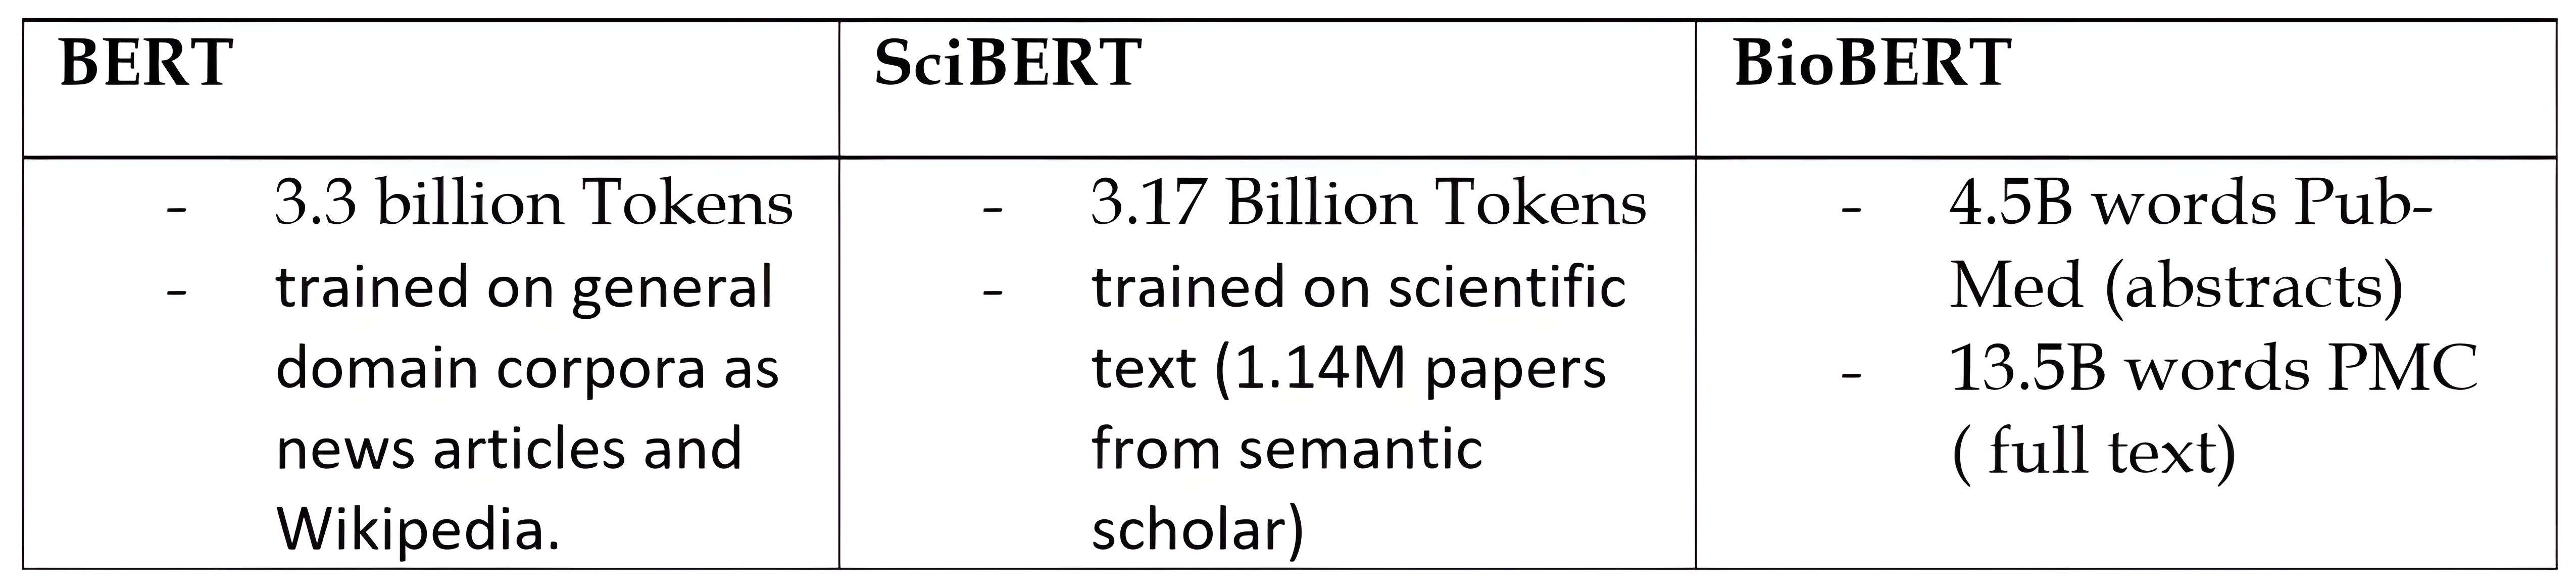
\includegraphics[width=1\textwidth]{4.graphics/figures/ch_5/BERT_Corpus}
	\label{fig:chapter03:setup}
\end{table}

For the task of software purpose classification, BERT model has been chosen because of the its merit over LSTM based models. Among verities of BERT particularly Sci-BERT is chosen because its training corpus is based on scientific-text which is more relevant for software purpose classification. In addition, Bio-BERT pre-trained model is also trained to compare performance with Sci-BERT. \\

The implementation of the software purpose classifier follows a previous project with SoMeSci dataset, SoMeNLP, which is a cascade of classifier modules for software, software-type and mention-type. Therefore, another module for software purpose classification is added on the top of previous cascade of classifier modules. A fully connected multi-class BERT classifier model implemented on this project is  shown on the figure below. 

\begin{figure}[htbp]
	\centering
	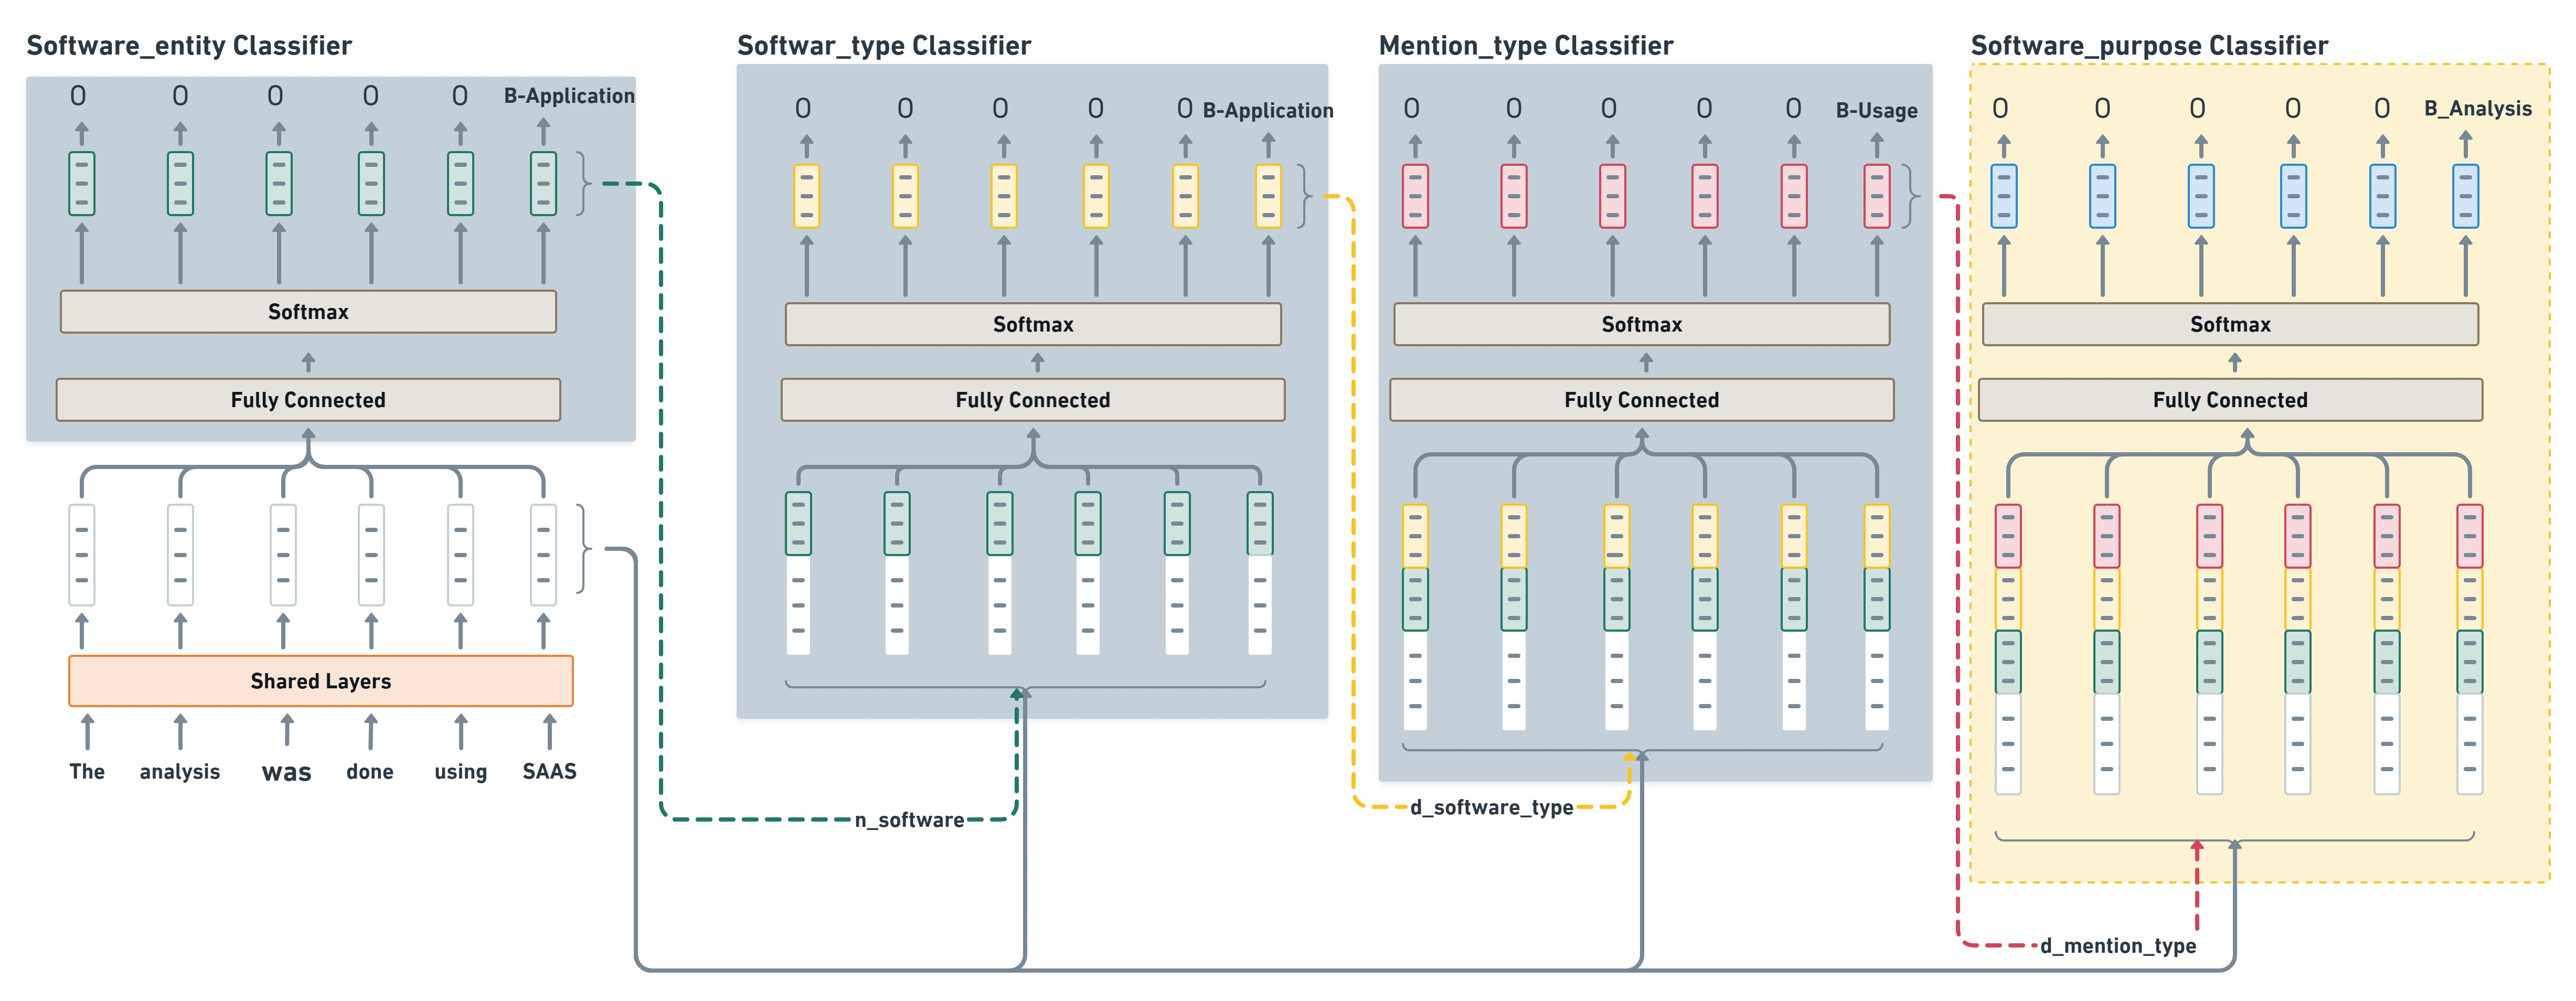
\includegraphics[width=1\textwidth]{4.graphics/figures/ch_5/fully_connected_model}
	\caption{Fully connected multi class 4-cascade classifier model for software, software-type, mention-type and software-purpose classification respectively.}
	\label{fig:chapter05:setup}
\end{figure}

 


